\documentclass[letterpaper]{article}
\usepackage{underscore}
\usepackage[left=2.0cm, right=2.0cm, top=2.0cm]{geometry}
\usepackage[utf8]{inputenc}
\usepackage{graphicx}
\usepackage{graphics}
\usepackage[spanish]{babel}
\usepackage{lipsum}
\usepackage{float}
\usepackage{subfigure}
\title{EV\_1\_6\_Explicar\_la\_operacion\_de\_los\_circuitos\_de\_activación\_con\_tiristores\_en\_convertidores\_CA-CD\_y\_CD-CA}
\author{Ledesma Hernandez Miguel Angel}
\date{20/09/2019}
\begin{document}
\maketitle
\vspace{9cm}
\begin{large}
\begin{center}

\includegraphics[width=4cm]{Imagenes/LOGO2.png}\\ \vspace{1.3cm}
\textbf{Universidad Politécnica de la Zona Metropolitana de Guadalajara}\\
\textbf{Sistemas Electrónicos de interfaz\\
Mecatrónica 4-A\\
}
\end{center}
\end{large}
\begin{Large}


\newpage
Comenzamos con la explicación de \textbf{¿Qué es un tristor?}\\
\vspace{.5cm}
En sintesis un tiristor es un componente electrónico que funciona como un relay con un diodo este necesita para funcionar dos condiciones: 
	\begin{itemize}
	 \item Se debe aplicar la intensidad de control en el terminal de la puerta, la intensidad debe cumplir con una amplitud y una duración determinada 
	 \item cuando se le aplique la intensidad de control en la terminal de la puerta, la intensidad del ánodo y cátodo debe ser positiva.
	\end{itemize}
Para identificar un tiristor en un diagrama debemos memorizar el siguiente simbolo: \\

\begin{figure}[hbtp]
\centering
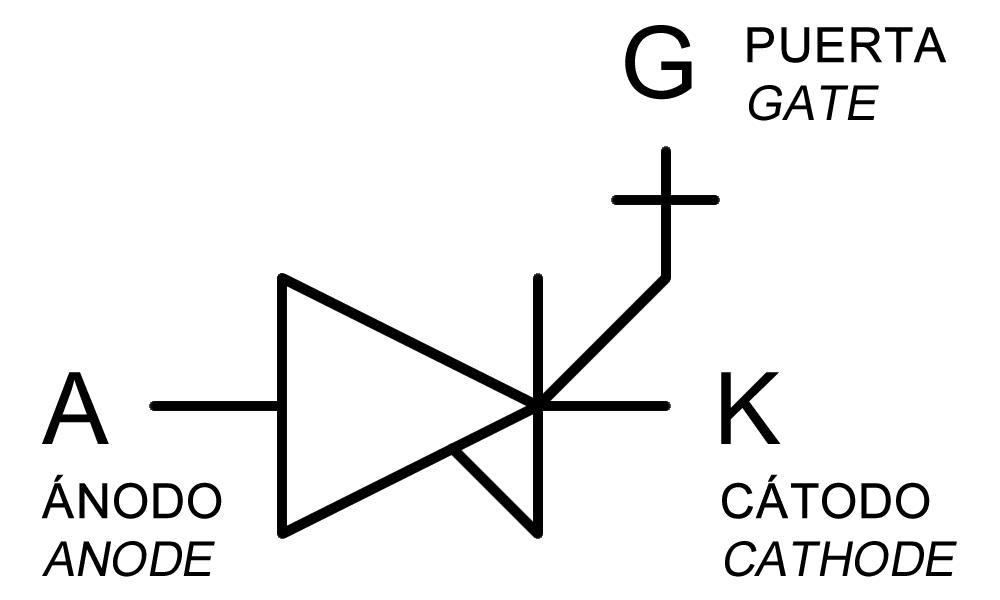
\includegraphics[scale=.2]{Imagenes/TiristorTC.png}\\
\caption{Tiristor}
\end{figure}

y podemos encontrar en forma física como: 

\begin{figure}[hbtp]
\caption{Tiristor}
\centering
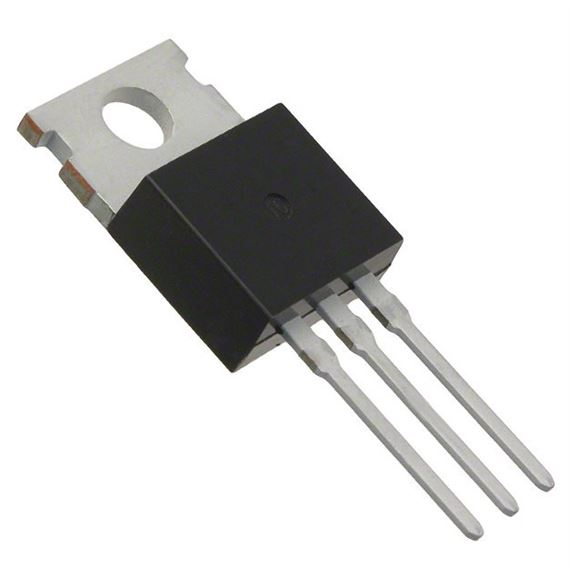
\includegraphics[scale=.3]{Imagenes/tiristor-2n6509.jpg}
\end{figure}

Este elemento tiene un estado de bloqueo[Cuando no hay una corriente que circule por el lemento] y un estado de conducción[Cunado cumple las condiciones y ahora si hay una corriente que circule el circuito]. Esta corriente se levanta de golpe y tal como funcionan los diodos rectifica la onda de manera que quede en una sola parte del plano cartesiano, como solo necesita que ándo y cátodo en positivo nos dará unicamente una onda positiva, como podemos ver en la siguiente figura.\\

\begin{figure}[hbtp]
\caption{onda del tristor}
\centering
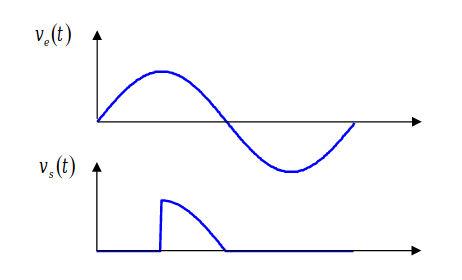
\includegraphics[scale=.5]{Imagenes/onda.png}
\end{figure}

Como podemos ver en la gáfica el la onda normal $V_e(t)$ es distinta a la onda de salida $V_s(t)$ esto sucede por que al cumplir las condiciones el componente deja pasar a la onda y como los diodos, cuando pasa por el negativo no permite el paso, por lo que lo toma y lo pasa como positivo. Así es como se genera esa onda que se asemeja a una aleta de tiburón. Tomando la onda negativa y poniendola en la posición según el tiristor y al cumplir las condiciones permitir el paso de una señal, para que cuando las condiciones ya no se cumplan, es decir cuando pase una señal negativa suceda lo que hace el diodo que es esperar a la onda positiva para poder hacer el proceso debeido. Esto si se encuentra en un circuito de corriente alterna [donde normalmente lo econtraremos[Sobre todo en los circuitos de alta tensión]].\\


Una vez entendido esto veamos como afecta a los circuitos CA-CD y CD-CA ya que podemos encontrar este circuito como puente de media onda semiconductor o puente de onda completa semiconductor.\\
\begin{figure}[hbtp]
\centering
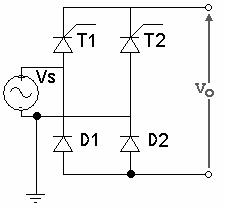
\includegraphics[scale=.5]{Imagenes/puente semi.png}\\
\caption{Puente semi conductor}
\end{figure}

Este tipo de puentes es para onda completa y tenemos puentes de media onda como podemos ver en la siguiente imagen.
\begin{figure}[hbtp]
\caption{Media onda}
\centering
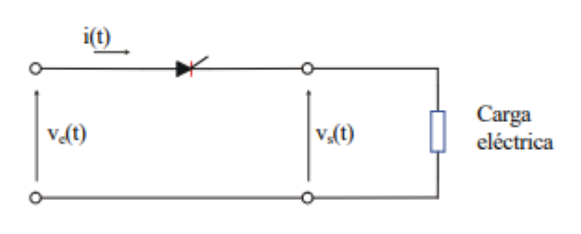
\includegraphics[scale=.5]{Imagenes/media.png}
\end{figure}\\

Este medio puente genera una onda que como ya hemos dicho se asemeja a una aleta de tiburón y esta onda se mantiene con respecto al tiempo siempre y cuando las condiciones que requieren los tiristores se cumplan.\\

Cuando se cumple la condición en la que el circuito es activado con cierto desfase en el ángulo $\alpha$ de la onda la corriente aumenta de manera mas lenta debido al inductor que estpa en el circuito. 
El voltaje de el circuito es positivo y se guarda dentro del inductor gracias a su campo magnetico. Pero llega un punto en el que el ciclo negativo desactiva el SRC y tambien el campo magnetico se descarga por medio la carga en sentido opuesto[Carga negativa] obteniendo voltaje negativo.\\

Con este componente tamiben podemos generar circuitos rectificadores de onda completa controlados\\
El circuito está basado en las leyes de Kirchoff esto por las mallas creadas por los transistores en la que se demuestra que ambos circuitos no pueden conducir al mismo tiempo asi que podemos decir que el $V_o$ es inverso al voltaje pico.
 \vspace{1.5cm}
\begin{center}
$V_o = V_{max}(1+cos \alpha)/p$
\end{center}
\newpage

Tambien encontramos rectificador monofasico controlado de tristores.\\
	y en este encontramos señales 
	\begin{itemize}
	 \item continua (En régimen permanente no se hace cero nunca)
	 \item discontinua (En régimen permanente se hace cero)
	\end{itemize}
	
	
En conclusión en componente rectifica la onda de una manera distinta pero parecida a los diodos rectificadores, de manera que la onda solo genera en sentido positivo y ademas de esto se generan ondas que son por así decirlo de un disparo en cuanto se cumplen las condiciones. Bien adaptado esto puede usarse para detectar presencia o ausencia de objetos, humedad... o también como ya se explicó en convertidores Ca-Cd y Cd-Ca.


\newpage
Bibliografía: 
 	


\end{Large}
\end{document}
